
%% bare_jrnl_compsoc.tex
%% V1.4b
%% 2015/08/26
%% by Michael Shell
%% See:
%% http://www.michaelshell.org/
%% for current contact information.
%%
%% This is a skeleton file demonstrating the use of IEEEtran.cls
%% (requires IEEEtran.cls version 1.8b or later) with an IEEE
%% Computer Society journal paper.
%%
%% Support sites:
%% http://www.michaelshell.org/tex/ieeetran/
%% http://www.ctan.org/pkg/ieeetran
%% and
%% http://www.ieee.org/

%%*************************************************************************
%% Legal Notice:
%% This code is offered as-is without any warranty either expressed or
%% implied; without even the implied warranty of MERCHANTABILITY or
%% FITNESS FOR A PARTICULAR PURPOSE! 
%% User assumes all risk.
%% In no event shall the IEEE or any contributor to this code be liable for
%% any damages or losses, including, but not limited to, incidental,
%% consequential, or any other damages, resulting from the use or misuse
%% of any information contained here.
%%
%% All comments are the opinions of their respective authors and are not
%% necessarily endorsed by the IEEE.
%%
%% This work is distributed under the LaTeX Project Public License (LPPL)
%% ( http://www.latex-project.org/ ) version 1.3, and may be freely used,
%% distributed and modified. A copy of the LPPL, version 1.3, is included
%% in the base LaTeX documentation of all distributions of LaTeX released
%% 2003/12/01 or later.
%% Retain all contribution notices and credits.
%% ** Modified files should be clearly indicated as such, including  **
%% ** renaming them and changing author support contact information. **
%%*************************************************************************


% *** Authors should verify (and, if needed, correct) their LaTeX system  ***
% *** with the testflow diagnostic prior to trusting their LaTeX platform ***
% *** with production work. The IEEE's font choices and paper sizes can   ***
% *** trigger bugs that do not appear when using other class files.       ***                          ***
% The testflow support page is at:
% http://www.michaelshell.org/tex/testflow/


\documentclass[10pt,journal,compsoc]{IEEEtran}
%
% If IEEEtran.cls has not been installed into the LaTeX system files,
% manually specify the path to it like:
% \documentclass[10pt,journal,compsoc]{../sty/IEEEtran}





% Some very useful LaTeX packages include:
% (uncomment the ones you want to load)


% *** MISC UTILITY PACKAGES ***
%
%\usepackage{ifpdf}
% Heiko Oberdiek's ifpdf.sty is very useful if you need conditional
% compilation based on whether the output is pdf or dvi.
% usage:
% \ifpdf
%   % pdf code
% \else
%   % dvi code
% \fi
% The latest version of ifpdf.sty can be obtained from:
% http://www.ctan.org/pkg/ifpdf
% Also, note that IEEEtran.cls V1.7 and later provides a builtin
% \ifCLASSINFOpdf conditional that works the same way.
% When switching from latex to pdflatex and vice-versa, the compiler may
% have to be run twice to clear warning/error messages.






% *** CITATION PACKAGES ***
%
\ifCLASSOPTIONcompsoc
  % IEEE Computer Society needs nocompress option
  % requires cite.sty v4.0 or later (November 2003)
  \usepackage[nocompress]{cite}
\else
  % normal IEEE
  \usepackage{cite}
\fi
% cite.sty was written by Donald Arseneau
% V1.6 and later of IEEEtran pre-defines the format of the cite.sty package
% \cite{} output to follow that of the IEEE. Loading the cite package will
% result in citation numbers being automatically sorted and properly
% "compressed/ranged". e.g., [1], [9], [2], [7], [5], [6] without using
% cite.sty will become [1], [2], [5]--[7], [9] using cite.sty. cite.sty's
% \cite will automatically add leading space, if needed. Use cite.sty's
% noadjust option (cite.sty V3.8 and later) if you want to turn this off
% such as if a citation ever needs to be enclosed in parenthesis.
% cite.sty is already installed on most LaTeX systems. Be sure and use
% version 5.0 (2009-03-20) and later if using hyperref.sty.
% The latest version can be obtained at:
% http://www.ctan.org/pkg/cite
% The documentation is contained in the cite.sty file itself.
%
% Note that some packages require special options to format as the Computer
% Society requires. In particular, Computer Society  papers do not use
% compressed citation ranges as is done in typical IEEE papers
% (e.g., [1]-[4]). Instead, they list every citation separately in order
% (e.g., [1], [2], [3], [4]). To get the latter we need to load the cite
% package with the nocompress option which is supported by cite.sty v4.0
% and later. Note also the use of a CLASSOPTION conditional provided by
% IEEEtran.cls V1.7 and later.





% *** GRAPHICS RELATED PACKAGES ***
%
\ifCLASSINFOpdf
  % \usepackage[pdftex]{graphicx}
  % declare the path(s) where your graphic files are
  % \graphicspath{{../pdf/}{../jpeg/}}
  % and their extensions so you won't have to specify these with
  % every instance of \includegraphics
  % \DeclareGraphicsExtensions{.pdf,.jpeg,.png}
\else
  % or other class option (dvipsone, dvipdf, if not using dvips). graphicx
  % will default to the driver specified in the system graphics.cfg if no
  % driver is specified.
  % \usepackage[dvips]{graphicx}
  % declare the path(s) where your graphic files are
  % \graphicspath{{../eps/}}
  % and their extensions so you won't have to specify these with
  % every instance of \includegraphics
  % \DeclareGraphicsExtensions{.eps}
\fi




% correct bad hyphenation here
\hyphenation{op-tical net-works semi-conduc-tor}

%my packages
\usepackage{cite}
\usepackage[table]{xcolor}
\usepackage{amsmath,amsfonts,multirow,graphicx,caption}
\usepackage{amsthm,amssymb}
\usepackage[ruled, vlined, linesnumbered, commentsnumbered, longend]{algorithm2e}

\usepackage[
n,
advantage,
operators,
sets,
adversary,
landau,
probability,
notions,
logic,
complexity,
asymptotics,
keys
] {cryptocode}
\usepackage[pdftex]{hyperref}
\hypersetup{
    colorlinks=true,
    linkcolor=blue,
    filecolor=magenta,  
    citecolor=blue,    
    urlcolor=cyan,
}
\usepackage{float}
\restylefloat{table}
\usepackage{tikz}

\usepackage{subfigure}
\usetikzlibrary{arrows, decorations.pathmorphing}


\newtheorem{theorem}{Theorem}[section]
\newtheorem{corollary}{Corollary}[theorem]
\newtheorem{lemma}[theorem]{Lemma}
\theoremstyle{definition}
\newtheorem{definition}{Definition}[section]

\begin{document}
% Do not put math or special symbols in the title.
\title{Accelerating Lattice based Proxy Re-Encryption
schemes on GPUs}
%
%
% author names and IEEE memberships
% note positions of commas and nonbreaking spaces ( ~ ) LaTeX will not break
% a structure at a ~ so this keeps an author's name from being broken across
% two lines.
% use \thanks{} to gain access to the first footnote area
% a separate \thanks must be used for each paragraph as LaTeX2e's \thanks
% was not built to handle multiple paragraphs
%
%
%\IEEEcompsocitemizethanks is a special \thanks that produces the bulleted
% lists the Computer Society journals use for "first footnote" author
% affiliations. Use \IEEEcompsocthanksitem which works much like \item
% for each affiliation group. When not in compsoc mode,
% \IEEEcompsocitemizethanks becomes like \thanks and
% \IEEEcompsocthanksitem becomes a line break with idention. This
% facilitates dual compilation, although admittedly the differences in the
% desired content of \author between the different types of papers makes a
% one-size-fits-all approach a daunting prospect. For instance, compsoc 
% journal papers have the author affiliations above the "Manuscript
% received ..."  text while in non-compsoc journals this is reversed. Sigh.

\author{Gyana~Sahu,
        Kurt~Rohloff
        % <-this % stops a space
\IEEEcompsocitemizethanks{\IEEEcompsocthanksitem G. Sahu and K. Rohloff are with the College of Computing Sciences, New Jersey Institute of Technology, New Jersey,
NJ, 07102.\protect\\
% note need leading \protect in front of \\ to get a newline within \thanks as
% \\ is fragile and will error, could use \hfil\break instead.
E-mail: see http://www.michaelshell.org/contact.html
}% <-this % stops an unwanted space
\thanks{Manuscript received April 19, 2005; revised August 26, 2015.}}

% note the % following the last \IEEEmembership and also \thanks - 
% these prevent an unwanted space from occurring between the last author name
% and the end of the author line. i.e., if you had this:
% 
% \author{....lastname \thanks{...} \thanks{...} }
%                     ^------------^------------^----Do not want these spaces!
%
% a space would be appended to the last name and could cause every name on that
% line to be shifted left slightly. This is one of those "LaTeX things". For
% instance, "\textbf{A} \textbf{B}" will typeset as "A B" not "AB". To get
% "AB" then you have to do: "\textbf{A}\textbf{B}"
% \thanks is no different in this regard, so shield the last } of each \thanks
% that ends a line with a % and do not let a space in before the next \thanks.
% Spaces after \IEEEmembership other than the last one are OK (and needed) as
% you are supposed to have spaces between the names. For what it is worth,
% this is a minor point as most people would not even notice if the said evil
% space somehow managed to creep in.



% The paper headers
\markboth{Journal of \LaTeX\ Class Files,~Vol.~14, No.~8, August~2015}%
{Shell \MakeLowercase{\textit{et al.}}: Bare Demo of IEEEtran.cls for Computer Society Journals}
% The only time the second header will appear is for the odd numbered pages
% after the title page when using the twoside option.
% 
% *** Note that you probably will NOT want to include the author's ***
% *** name in the headers of peer review papers.                   ***
% You can use \ifCLASSOPTIONpeerreview for conditional compilation here if
% you desire.



% The publisher's ID mark at the bottom of the page is less important with
% Computer Society journal papers as those publications place the marks
% outside of the main text columns and, therefore, unlike regular IEEE
% journals, the available text space is not reduced by their presence.
% If you want to put a publisher's ID mark on the page you can do it like
% this:
%\IEEEpubid{0000--0000/00\$00.00~\copyright~2015 IEEE}
% or like this to get the Computer Society new two part style.
%\IEEEpubid{\makebox[\columnwidth]{\hfill 0000--0000/00/\$00.00~\copyright~2015 IEEE}%
%\hspace{\columnsep}\makebox[\columnwidth]{Published by the IEEE Computer Society\hfill}}
% Remember, if you use this you must call \IEEEpubidadjcol in the second
% column for its text to clear the IEEEpubid mark (Computer Society jorunal
% papers don't need this extra clearance.)

% for Computer Society papers, we must declare the abstract and index terms
% PRIOR to the title within the \IEEEtitleabstractindextext IEEEtran
% command as these need to go into the title area created by \maketitle.
% As a general rule, do not put math, special symbols or citations
% in the abstract or keywords.
\IEEEtitleabstractindextext{%
\begin{abstract}
Proxy Re-Encryption (PRE) is an indispensable tool in many public-key cryptographic schemes that enables users to delegate decryption rights to other users via a proxy. In this work, we present a high performance implementation of PRE schemes on NVIDIA GPUs. We target two lattice based PRE schemes, BV-PRE and Ring-GSW PRE defined over polynomial rings. We design a parallel Number Theoretic Transform (NTT) procedure capable of working on arbitrary precision moduli (in CRT form) and demonstrate several low level and GPU optimizations techniques to accelerate the PRE schemes.  

For the same or higher security settings our results show 39x to 228x factors of improvement in performance with a peak throughput of 6.3 Mbps when compared to the CPU implementation of the BV-PRE scheme in the PALISADE lattice crypto software library. Similarly, for the Ring-GSW PRE scheme we achieve a peak throughput of 49 Mbps and up to 11x improvement in performance.  
\end{abstract}

% Note that keywords are not normally used for peerreview papers.
\begin{IEEEkeywords}
Applied Cryptography, GPU, Hardware Acceleration.
\end{IEEEkeywords}}


% make the title area
\maketitle


% To allow for easy dual compilation without having to reenter the
% abstract/keywords data, the \IEEEtitleabstractindextext text will
% not be used in maketitle, but will appear (i.e., to be "transported")
% here as \IEEEdisplaynontitleabstractindextext when the compsoc 
% or transmag modes are not selected <OR> if conference mode is selected 
% - because all conference papers position the abstract like regular
% papers do.
\IEEEdisplaynontitleabstractindextext
% \IEEEdisplaynontitleabstractindextext has no effect when using
% compsoc or transmag under a non-conference mode.


\IEEEpeerreviewmaketitle


% Computer Society journal (but not conference!) papers do something unusual
% with the very first section heading (almost always called "Introduction").
% They place it ABOVE the main text! IEEEtran.cls does not automatically do
% this for you, but you can achieve this effect with the provided
% \IEEEraisesectionheading{} command. Note the need to keep any \label that
% is to refer to the section immediately after \section in the above as
% \IEEEraisesectionheading puts \section within a raised box.
\input{introduction}

\section{Design} \label{sec:design}

\subsection{Syntax of unidirectional PRE Scheme}
We recall that a non-interactive PRE scheme is an ensemble of PPT algorithms $\Pi = $ (\emph{ParamsGen, KeyGen, ReKeyGen, Encrypt, ReEncrypt, Decrypt}), which can be defined as per the following syntax:

\begin{itemize}
\item{\textbf{ParamsGen$\left( 1^\lambda\right)$}}: It takes the security parameter $\lambda$ and returns the corresponding public parameters \textit{pp}.

\item{\textbf{KeyGen$\left( pp, 1^\lambda\right)$}}: It takes the public parameters $pp$ and returns the key pair $\left(pk,sk \right)$.

\item{\textbf{ReKeyGen}$\left(pp, sk_i,pk_j \right)$}: It takes the public parameters, secret key of publisher $i$, public key of subscriber $j$ and returns the re-encryption key $rk_{i \rightarrow j}$.

\item{\textbf{Encrypt$\left(pp,pk,m \right)$}}: Given public key and public parameters, it encrypts the message $m$ and returns a ciphertext $c$.

\item{\textbf{ReEncrypt}$\left( pp, rk_{i\rightarrow j},c_i \right)$}: It transforms a ciphertext $c_i$ of the party $i$ into a ciphertext $c_j$ that can be decrypted by party $j$.

\item{\textbf{Decrypt}$\left(pp,sk,c\right)$}: It recovers the message $m$ from ciphertext $c$.

\end{itemize}

\section{Preliminaries and Mathematical Notations} \label{sec:prelims}
In this work, we represent scalars in plain, vectors by lower-case bold letters (e.g., $\mathbf{a}$) and matrices by upper-case bold letters (e.g., $\mathbf{A}$). Ring elements, for example  $x \in R_q$, are represented by lower case letters in plain. We define $\left[k\right] = \left\{1, \cdots , k\right\}$ for any non-negative integer $k$. The $i$-th norm of a vector $\vec{\mathbf{v}}$ is denoted by $\norm{\mathbf{v}}_i$. We denote the tensor (Kronecker) product of two matrices $\mathbf{A}$ and $\mathbf{B}$ as $\mathbf{A} \otimes \mathbf{B}$. We extend this notation to a vector $\vec{\mathbf{v}}$ where the Kronecker product is represented as  $\vec{\mathbf{v}} \otimes \mathbf{A}$. Unless explicitly mentioned logarithms are to be understood with base 2. We denote the horizontal and vertical concatenation of matrices by operators $\left(\cdot||\right)$  and $\left( \cdot ||^\intercal \right)$ respectively. For two matrices $\mathbf{A},\mathbf{B} \in \mathbb{Z}^{n \times n}$ $\left[ \mathbf{A} \; || \; \mathbf{B} \right]$ produces a matrix $\mathbf{C} \in \mathbb{Z}^{n \times 2n}$. Similarly, $\left[ \mathbf{A} \; ||^\intercal \; \mathbf{B} \right]$ produces a matrix $\mathbf{C} \in \mathbb{Z}^{2n \times n}$.


\subsection{Gadget Matrix and Relinearization functions:}

For LWE dimension $n$ and modulus $q$, we use the following ``gadget'' vector \cite{micciancio2012trapdoors}: 
$$\mathbf{g} = \left(1,2,4,\cdots,2^{\ell-1} \right) \in \mathbb{Z}_q^{\ell}, \text{ where } \ell = \lceil \log q \rceil.$$
The \emph{gadget matrix} \textbf{G} is then defined as the diagonal concatenation of the \textbf{g} vector $n$ times. Formally, it is written as $ \mathbf{G} = \mathbf{g} \otimes I_n \in \mathbb{Z}_q^{\ell n\times n}$. To perform relinearization we define the following operations \cite{brakerski2011fully, gentry2013homomorphic} with respect to an element $a$ which can be either a vector or matrix or polynomial ring. 

\begin{itemize}
\item{$\mathbf{BitDecomp}\left(a\right)$}: For a vector $\vec{\mathbf{a}} \in \mathbb{Z}_q^n$ this operation produces a bit decomposed and expanded vector $\vec{\mathbf{a}}' \in \mathbb{Z}_q^{n\ell}$ where $a_i = \sum^{\ell}_{j=0}2^j a'_{i\ell + j}$. In case of a matrix $\mathbf{A} \in \mathbb{Z}_q^{m\times n}$ this operation produces a matrix that is expanded along the column resulting in $\mathbf{A}' \in \mathbb{Z}_q^{m\times n\ell}$. Finally, in case of a polynomial ring $a \in R_q$ this operation produces $\mathbf{a}' \in R_q^\ell$.  
\item{$\mathbf{PowerOf2}\left(a\right)$}: Given a vector $\vec{\mathbf{a}} \in \mathbb{Z}_q^n$ this operation produces an expanded vector $\vec{\mathbf{a}}' \in \mathbb{Z}_q^{n\ell}$ where $\vec{\mathbf{a}}' = \left(a_0,2a_0,\cdots,2^{\ell-1}a_0,\cdots, 2^{\ell-1}a_{n-1}\right)$. Similarly, for a polynomial ring $a \in R_q$ we get $\vec{\mathbf{a}}' \in R_q^{\ell}$ where $a'_i = 2^ia$.
\end{itemize}
Using these operations, we can produce a product of $\vec{\mathbf{a}}$ and $\vec{\mathbf{b}}$ as follows: $$\left\langle \mathbf{BitDecomp}\left( \vec{\mathbf{a}} \right), \mathbf{PowersOf2}\left( \vec{\mathbf{b}}\right)\right\rangle = \left\langle \vec{\mathbf{a}},\vec{\mathbf{b}}\right\rangle$$ 


\section{Number Theoretic Transform and Bit-Decomposition} \label{sec:lowerMath}

\subsection{Number Theoretic Transform}

Cryptosystems based on the RLWE security assumption are defined over a polynomial ring $R = \mathbb{Z}\left[ X \right] / \Phi_m\left( X\right) $ where $\Phi_m\left( X\right)$ is an irreducible monic cyclotomic polynomial of order $m$. This notation is extended to a polynomial $R_q$ modulo an integer $q$ where the coefficients of the polynomial are in the interval
$\left(-q/2,q/2\right]$. Alternatively, an element $a \in R_q$ is simply considered to be a coefficient vector $\vec{\mathbf{a}} \in \mathbb{Z}_q^{\varphi\left( m \right)}$. While addition of these polynomials is quite efficient, multiplication leads to quadratic time complexity. To circumvent this inefficiency, we represent polynomial rings in the so called ``Evaluation'' representation. For a polynomial $a \in R_q$ the coefficients can be converted to the evaluation domain $\bar{a}$ by evaluating $a\left(X\right)$ at each of the $m$-th primitive roots of unity modulo $q$. The coefficients of $\bar{a}$ are related to polynomial $a$ through the relation $\bar{a}_i = a\left( \omega^i \right) \text{ mod } q$ where $\left(i,m\right)=1$ and $\omega$ is a $m$-th primitive root of unity modulo $q$. 

This back and forth conversion of a polynomial can be achieved efficiently by using number theoretic transforms (NTT) which is roughly similar to the classical $n$-dimensional fast Fourier transform where a finite field is used instead of complex numbers. Concretely, in our implementation, we use the power of two cyclotomics ($m = 2^k$) where $\Phi_m\left(X\right)$ is maximally sparse and the ring dimension $n = \varphi\left( m\right) = m/2$ is also a power of two. The power of two cyclotomics along with NTT has become so pervasive in lattice based cryptography that the overall efficiency of the cryptosystem depends upon the latency of NTT procedure. For this reason, we chose to implement NTT as an iterative Cooley-Tukey algorithm. More specifically, we implemented the NTT routine with Fermat theoretic transform (FTT) optimization which eliminates interleaved zero paddings when using the conventional NTT procedure.

\subsection{Parallel NTT}

Exploiting the NVIDIA GPU architecture, we reduce the NTT latency further by mapping the butterfly computations of each of the $\log{n}$ stages to an independently processing thread of a thread block. In the NVIDIA CUDA architecture, each kernel or device function can be potentially divided into a $3$-dimensional array of blocks where a block further consists of several threads. Because of hardware restrictions, a maximum of $1024$ threads can be assigned to a block. Further, the threads within a block have the capability to share data and more importantly synchronize with each other. In our implementation, for small polynomials ($n \leq 1024$) we map the coefficients entirely to a thread block and synchronize the thread block after completion of a stage as shown in Figure \ref{fig:gpuNTT}. We use shared memory for storing the intermittent results as latency associated with global memory is higher than that of shared memory which resides on the chip. For larger polynomial rings ($n>1024$), we use a combination of block level synchronization and  stream level synchronization to avoid data race conditions. As stream level synchronization avoids data race conditions via global memory synchronization we pay the penalty of using slower memory but only for a fraction of the NTT procedure calls.

The evaluation of the proposed NTT procedure on GPU platforms and CPU platforms is shown in Figure \ref{fig:cpugpuRunTimes}. From the figure, we can see that the CPU platform running on a single thread achieves slightly better performance for smaller ring dimensions. As the ring dimensions grow higher we can see that the GPU platform starts showing significant improvement in performance. 

\begin{figure}	
\centering
\resizebox{5cm}{6cm}{%
    
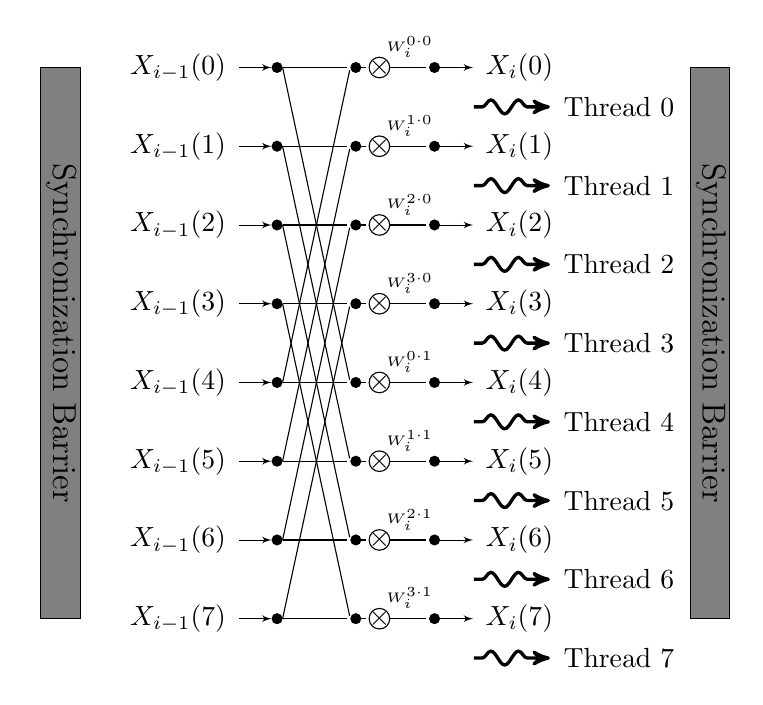
\begin{tikzpicture}[scale = 1, node distance=0.3cm, auto, ->,    > = stealth',
       shorten > = 1pt,decoration = {snake,   % <-- added
                    pre length=3pt,post length=7pt,% <-- for better looking of arrow,
                    }]
                    
\tikzstyle{n}= [circle, fill, minimum size=4pt,inner sep=0pt, outer sep=0pt]
\tikzstyle{mul} = [circle,draw,inner sep=-1pt]
\tikzstyle{thd} = [draw=blue, very thick, decorate]

% Define two helper counters
\newcounter{x}\newcounter{y}
              
    \foreach \y in {0,...,7}
        \node[n, pin={[pin edge={latex'-,black}]left:$X_{i-1}(\y)$}]
              (N-0-\y) at (0,-\y) {};
              
    % draw connector nodes
    \foreach \y in {0,...,7}
        \foreach \x / \c in {1/1}
            \node[n, name=N-\c-\y] at (\x,-\y) {};
            
   % Draw outputs
    \foreach \y in {0,...,7}
        \node[n, pin={[pin edge={-latex',black}]right:$X_i(\y)$}]
              (N-3-\y) at (2,-\y) {};         

            
    % draw x nodes
    \foreach \y in {0,...,7}
        \foreach \x / \c  in {1/2}
            \node[mul, right of=N-\x-\y] (N-\c-\y) {${\times}$};                
            
    % horizontal connections 
 \foreach \y in {0,...,7}
        \foreach \x / \c in {0/1,1/2}
        {
            \path (N-\x-\y) edge[-] (N-\c-\y);
       }  
       
      % Draw the W_8 coefficients
    \setcounter{y}{0}
    \foreach \i / \j in {0/0,1/0,2/0,3/0,0/1,1/1,2/1,3/1}
    {
        \path (N-2-\arabic{y}) edge[-] node {\tiny $W^{\i\cdot\j}_{i}$}
              (N-3-\arabic{y});
        \addtocounter{y}{1}
    }  
    
    % Connect nodes
    \foreach \sourcey / \desty in {0/4,1/5,2/6,3/7,
                                   4/0,5/1,6/2,7/3}
       \path (N-0-\sourcey.east) edge[-] (N-1-\desty.west); 
       
       
 %draw sync rectangle
 \draw[draw=black, fill=gray, name=sync1] (-3,0) rectangle (-2.5,-7);
 \node[ label = {[rotate=-90,font=\large] Synchronization Barrier}] at (-3.05,-3.5) {};

% Draw outputs
\foreach \y in {0,...,7}
	\path[draw=black, very thick, decorate] (2.5,-\y-0.5) -- (3.5,-\y-0.5) node[right] {Thread \y};
	
 %draw sync rectangle
 \draw[draw=black, fill=gray, name=sync2] (5.25,0) rectangle (5.75,-7);	
 \node[ label = {[rotate=-90,font=\large] Synchronization Barrier}] at (5.2,-3.5) {}; 
         

  \end{tikzpicture}
  } %end of resizebox
  \caption{Parallel implementation of the $i$-th stage of NTT on a GPU, $N=8$. }
\label{fig:gpuNTT}
\end{figure} 

%\begin{figure}
%\centering
%\resizebox{\linewidth}{6cm}{
%\includegraphics{"gnu-ntt-runTimeComparison"}
%}
%\caption{Comparison of CPU and GPU runtimes of NTT algorithm.}
%\label{fig:cpugpuRunTimes}
%\end{figure}

\begin{figure}
\centering
\begin{tikzpicture}
\begin{axis}[
xlabel={Ring dimension, $N=2^k$},
ylabel=Runtime (in ms),
grid=major,
ybar,
bar width = 7pt,
xtick=data,
width=12cm, height=7cm,
legend pos=north east,
legend style={ at={(0.85,0.95)}},
]
\addplot[pattern=crosshatch, pattern color=blue!50] table [x=xcod, y=GTX]   {CPUVSGPU-OnDimension};
\addplot[pattern=north east lines, pattern color=red!80] table [x=xcod, y=CPU] {CPUVSGPU-OnDimension};
\addplot[pattern=crosshatch dots, pattern color=orange!150] table [x=xcod, y=RTX] {CPUVSGPU-OnDimension};
\legend{GPU-GTX 1050, CPU-i7-7700HQ, GPU-Titan RTX};
\end{axis}
\end{tikzpicture}
\caption{Comparison of CPU and GPU runtimes of the NTT algorithm.}
\label{fig:cpugpuRunTimes}
\end{figure}

\subsection{Barrett Modulo Reduction and Arbitrary Precision Support}

For modulo reduction, we used a variation of the generalized Barrett modulo reduction  \cite{dhem1998recent} as outlined in Algorithm \ref{algo:modBarrett}. Barrett modulo reduction requires a pre-computation term $\mu = \lfloor 2^{2b} / q\rfloor$ for a particular modulus $q$ and its bit width, $b = \lceil \log_2{q}\rceil$. We pre-compute these terms and transfer them to GPU global memory for read only access to any kernel. NVIDIA GPUs are restricted to a $32$-bit architecture and $64$-bit arithmetic are supported only through assembly code emulation. For this reason, we prefer moduli with bit width closer to $32$-bits so that the precomputation term $\mu$ fits into the word size. Concretely, we allow up to $29-30$ bit width moduli in our implementation. 

Lattice based cryptosystems employ the addition of low norm noise terms to base their security on Ring-LWE and LWE assumptions. For preserving the correctness constraints so that ciphertexts are decrypted correctly, the modulus $q$ should be chosen large enough such that the final accumulated error terms do not ``wrap around'' modulo $q$. To extend support for larger moduli we store a set of increasing prime moduli $q_i$ by an application of the Chinese Remainder Theorem (CRT). We only reconstruct the coefficients into larger terms for the purpose of decryption or bit-decomposition where the polynomial needs to be represented in terms of the larger modulus, $q = \prod_{i=0}^{t-1} q_i$.

Evaluation of the NTT procedure on a GPU with varying number of moduli, $t$ and ring dimension $N$ can be seen in Figure \ref{fig:gpuRunTimesOnModuli}. For most of the ring dimensions, the runtimes vary a little. This is due to the fact that GPUs have the capability to improve throughput by hiding latency with the concurrent execution of the NTT procedure on different polynomials. On a CPU platform the runtime is estimated to scale linearly with the number of moduli assuming a single thread execution environment.

%Graph replace by pgfplot, looks better now!
%\begin{figure}
%\centering
%\includegraphics[height=6cm, width=\linewidth]{"gnu-ntt-runTime-dimension-t"}
%\caption{GPU runtimes of NTT algorithm with varying dimension and moduli, $t$.}
%\label{fig:gpuRunTimesOnModuli}
%\end{figure}


\begin{figure}
\centering
\begin{tikzpicture}
\begin{axis}[
xlabel={Number of moduli, $t$},
ylabel=Runtime (in ms),
grid=major,
width=10cm, height=7cm,
legend pos = outer north east,
]
\addplot+[smooth] table [x=x, y=y1]   {GPURuntimesForCRT};
\addplot+[smooth] table [x=x, y=y2]   {GPURuntimesForCRT};
\addplot+[smooth] table [x=x, y=y3]   {GPURuntimesForCRT};
\addplot+[smooth] table [x=x, y=y4]   {GPURuntimesForCRT};
\addplot+[smooth] table [x=x, y=y5]   {GPURuntimesForCRT};
\addplot+[smooth] table [x=x, y=y6]   {GPURuntimesForCRT};
\addplot+[smooth] table [x=x, y=y7]   {GPURuntimesForCRT};
\legend{$N=2^9$,$N=2^{10}$,$N=2^{11}$,$N=2^{12}$,$N=2^{13}$, $N=2^{14}$, $N=2^{15}$ };
\end{axis}
\end{tikzpicture}
\caption{GPU runtimes of the NTT algorithm with varying dimension $N$ and moduli $t$.}
\label{fig:gpuRunTimesOnModuli}
\end{figure}  



\begin{algorithm}
\caption{Mod Barrett Reduction}
\label{algo:modBarrett}
	\SetAlgoLined
	\SetKw{KwBy}{by}
	\SetKwInOut{KwIn}{Input}
	\SetKwInOut{KwOut}{Output}
	\KwIn{ $x \in \left[0, \left(q-1\right)^2\right]$, modulus $q$, bit-width $b = \lceil \log{q} \rceil$, $\bar{q} = 2\cdot q$ and $\mu = \lfloor 2^{2b}/q \rfloor$.}
	\KwOut{$z \gets x \% \; q$ }
	$z \gets x \gg b$ \;
	$z \gets z\cdot \mu$ \;
	$z \gets z \gg b$ \;
	$z \gets z\cdot q$ \; 
	$x \gets x - z$ \;
	\If{ $x >= \bar{q}$}{$z \gets x-\bar{q}$\; }
	\If{ $z >= q$}{$z \gets z-q$\; }
\KwRet{$z$}
\end{algorithm}

\subsection{Bit Decomposition} \label{subsec:bit-decomp}

Bit decomposition along with the relinearization procedure forms the backbone of lattice based cryptography. While bit decomposing integers is simple in finite field arithmetic, it is accompanied with additional overheads in Ring-LWE based cryptosystems. In Ring-LWE cryptosystems, ciphertexts and other key elements are mostly present in evaluation representation. To bit decompose, polynomial rings need to be switched back to coefficient representation. At this stage, bit decomposition of the polynomial results in a vector of $b$ polynomials, where $b$ is the bit length of the modulus $q$. To perform further computations, these polynomials need to be converted back to evaluation representation by a series of NTT calls. Since the bit decomposed polynomials are independent of each other, we apply NTT procedures on them in parallel using a three dimensional CUDA grid mapping. To avoid race conditions in the NTT procedure, we provide the kernel with appropriate synchronization.  From Figure \ref{fig:gpuVScpuBitDecomp}, we can observe that our GPU implementation of bit decomposition outperforms runtimes of the CPU platform for all ring dimensions and further the speedups are more pronounced in case of higher ring dimensions. 

%\begin{figure}
%\centering
%\resizebox{\linewidth}{6cm}{
%%height=8cm, width=9cm
%\includegraphics[]{"gnu-vs-cpu-BitDecomp"}
%}
%\caption{GPU vs CPU runtimes of bit decomposing polynomial ring with varying ring dimension, $N$.}
%\label{fig:gpuVScpuBitDecomp}
%\end{figure} 

\begin{figure}
\centering
\begin{tikzpicture}
\begin{axis}[
xlabel={Ring dimension, $N=2^k$},
ylabel=Runtime (in ms),
grid=major,
ybar,
bar width = 5pt,
xtick=data,
width=12cm, height=7cm,
legend style={ 
	at={(0.85,0.96)},
},
]
\addplot[pattern=crosshatch, pattern color=blue!50] table [x=x, y=y1]   {GPUvsCPUBitDecomp};
\addplot[pattern=north east lines, pattern color=red!80] table [x=x, y=y2] {GPUvsCPUBitDecomp};
\addplot[pattern=crosshatch dots, pattern color=orange!150] table [x=x, y=y3] {GPUvsCPUBitDecomp};
\legend{GPU-GTX 1050, CPU-i7-7700HQ, GPU-Titan RTX};
\end{axis}
\end{tikzpicture}
\caption{GPU vs CPU runtimes of bit decomposing a polynomial ring with varying ring dimension $N$.}
\label{fig:gpuVScpuBitDecomp}
\end{figure} 





\section{PRE Cryptosystem with BV FHE scheme} \label{bvpre}

The BV-PRE \cite{polyakov2017fast} scheme described here is based on the BV FHE \cite{brakerski2011fully} scheme introduced by Brakerski and Vaikuntanathan. The message space for the scheme is restricted to $\mathcal{M} \in R_p$ where $p$ is the plaintext modulus.

\subsection{BV Encryption Scheme}

The scheme is parameterized using the following quantities:

\begin{itemize}
\item Security parameter $\left( \lambda \right)$,
\item Ciphertext modulus $q$ and plaintext modulus $2 \leq p \ll q$,
\item Ring dimension $n$,
\item $D$-bounded discrete Gaussian error distribution $\chi_e$ with distribution parameter $\sigma_e$,
\item Ternary uniform distribution $\mathcal{T}$ which samples from  $\left\{ -1, 0, 1 \right\}$, 
\item Discrete uniform distribution $\mathcal{U}_q$,
\end{itemize}


The scheme consists of the following operations:

\noindent \textbullet\ \textbf{ParamsGen$\left(1^\lambda\right)$}: Choose positive integers $q = q\left(\lambda\right)$ and $n = n\left( \lambda \right)$. Return $pp = \left(p,q,n\right)$.\\
\noindent \textbullet\ \textbf{KeyGen$\left(pp, \lambda \right)$}: Sample polynomials $a \sample \mathcal{U}_q$, $s \sample \mathcal{T}$ and $e \sample \chi_e$. Compute $b := a\cdot s + pe \in R_q$. Set the public key $pk$ and private key $sk$ as follows: $$sk := \left( 1,s \right) \in R_q^2, \; pk := \left(a,b\right) \in R_q^2$$
\noindent \textbullet\ \textbf{Encrypt$\left(pp, pk = \left(a,b\right), m \in \mathcal{M} \right)$}: Sample polynomials $v \sample \mathcal{T}, e_0, e_1 \sample \chi_e$. Compute the ciphertext $c = \left( c_0,c_1 \right) \in R_q^2$ as follows: $$c_0 = b\cdot v + pe_0 +m \in R_q, \; c_1 = a\cdot v + pe_1 \in R_q$$
\noindent \textbullet\ \textbf{Decrypt}$\left(pp, sk = s, c = \left(c_0,c_1\right) \right)$:  Compute the ciphertext error $ t = c_0 - s \cdot c_1 \in R_q$. Output $m' = t  \text{ mod } p$. For correct decryption, the coefficients of the noise polynomial, $t$ should not wrap around modulo $q$.

\subsection{Proxy Re-Encryption Scheme}

We refer to the publisher of information as party A and the subscriber of information via the proxy as party B. Additional operations pertaining to PRE computation are as follows:\\

\noindent \textbullet\ \textbf{Preprocess}$\left(pp,\lambda, sk_B = \left(1,s_B \right) \right)$ Sample uniformly distributed random polynomials $\alpha_i \sample \mathcal{U}_q$ and error polynomials $e_i \sample \chi_e$ for $i \in \left[0, \; \lceil \log_2(q)/r\rceil \right)$. Here $r$ is the relinearization window. Compute the following elements:
\begin{align*}
\gamma_i = \alpha_i\cdot s_B + pe_i \in R_q;  \; pk_B = \left( \alpha_i, \gamma_i \right)_{i \in \left\{0,1,\cdots, \lfloor \log_2(q)/r\rfloor  \right\}}
\end{align*}
\noindent \textbullet\ \textbf{ReKeyGen}$\left(pp, sk_A = \left(1,s_A\right), pk_B\right)$: Compute $\beta_i$ and set the re-encryption key as follows:
$$\beta_i = \gamma_i - s_A\cdot (2^r)^i \in R_q, \; rk_{A\rightarrow B} = \left( \alpha_i, \beta_i \right)_{i \in \left\{0,1,\cdots, \lfloor \log_2(q)/r\rfloor  \right\}}$$
\noindent \textbullet\ \textbf{ReEncrypt}$\left(pp, rk_{A\rightarrow B} = \left(\alpha_i,\beta_i\right), c = \left(c_0,c_1 \right) \right)$: To get the re-encrypted ciphertext $c' = \left(c_0',c_1' \right)$ first apply $2^r$ base decompositions and proceed as follows:
\begin{align*}
c_0' = c_0 + \sum_{i=0}^{\lfloor \log_2{(q)}/r \rfloor} \left( c_1^{\left(i \right)} \cdot \beta_i \right) , \; c_1' = \sum_{i=0}^{\lfloor \log_2{(q)}/r \rfloor} \left( c_1^{\left(i \right)} \cdot \alpha_i \right)
\end{align*}
where $c_1^{\left( i \right)}$ represents the $i$-th digit of the base-$2^r$ decomposition of $c_1$.\\


Under the new secret key $sk = \left(1, s_B\right)$ decryption of the ciphertext $c' = \left(c_0',c_1'\right)$ can be shown as
\begin{align*}
c_0' - s_B\cdot c_1' & = c_0 + \sum_{i=0}^{\lfloor \log_2{(q)}/r \rfloor} \left( c_1^{\left(i \right)} \cdot \beta_i \right) - s_B \cdot \sum_{i=0}^{\lfloor \log_2{(q)}/r \rfloor} \left( c_1^{\left(i \right)} \cdot \alpha_i \right) \\
& = c_0 + \sum_{i=0}^{\lfloor \log_2{(q)}/r \rfloor}\left( c_1^{\left(i \right)} \cdot \left\{ \alpha_i\cdot s_B + pe_i - s_A\cdot \left(2^r \right)^i \right\} \right) \\ 
  &  \hskip 0.3\linewidth - s_B\cdot \sum_{i=0}^{\lfloor \log_2{(q)}/r \rfloor} \left( c_1^{\left(i \right)} \cdot \alpha_i \right) \\
& = c_0 - s_A\cdot c_1 + pE_i; \; E_i = \sum_{i=0}^{\lfloor \log_2{(q)}/r \rfloor} \left( c_1^{\left( i \right)} \cdot e_i \right) 
\end{align*}

To preserve the correctness of the re-encrypted ciphertext $c'=\left(c_0',c_1'\right)$, we derive the following constraint:
\begin{align*}
\norm{t}_\infty & \leq 3\sqrt{n}pD +  \sqrt{n}pD\cdot D_r {\lceil \log_2{(q)}/r \rceil} \\ & \approx \sqrt{n}p D D_r \left( {\lceil \log_2{(q)}/r \rceil}+1\right) \ni r > 1
\end{align*} 
$$ \Rightarrow q \geq 2\sqrt{n}p DD_r \left({\lceil \log_2{(q)}/r \rceil} +1\right) $$
where, $D_r$ is the bound of the bit decomposed polynomial in base $2^r$ representation.
\subsection{Security}
The security of PRE schemes is generally covered under indistinguishability against chosen-plaintext attacks (\indcpa). For brevity we omit the formal definition of the \indcpa\ security notion and capture the security with the following theorem. 
\begin{theorem} \cite{polyakov2017fast} Under the $\mathbf{RLWE}_{\Phi,q,\chi_e}$ assumption, the BV-PRE scheme is $\indcpa$ secure. Specifically, for a poly-time adversary $\adv$, there exists a poly-time distinguisher $\ddv$ such that 
$$\text{Adv}^{cpa}_{\adv}\left(\lambda \right) \leq \left( \rho\cdot\left(Q_{rk}+Q_{re}\right)+ N + 1\right)\cdot\text{Adv}^{\mathbf{RLWE}_{\Phi,q,\chi}}_{\ddv}$$ 

\noindent where $Q_{rk}$ and $Q_{re}$ are the numbers of re-encryption key queries and re-encryption queries, respectively; N is the number of honest entities; $\lambda$ is the security parameter; $\Phi$ is the cyclotomic polynomial defining the ring $R_q = \mathbb{Z}_q[x]/\langle \Phi\rangle$ and $\rho = \lceil \log_2{ (q) }/r\rceil$. 
\end{theorem}

\section{PRE Cryptosystem with Ring-GSW FHE scheme} \label{rgswpre}

The Ring-GSW PRE scheme described here is based on the Ring-GSW FHE  scheme, a RLWE variant of the GSW \cite{gentry2013homomorphic} FHE scheme. The message space for the scheme is restricted to $\mathcal{M} \in R_p$ similar to the BV-FHE scheme.

\subsection{Ring-GSW Encryption Scheme}

The scheme is parameterized similar to the BV-FHE scheme. It consists of the following operations:

\noindent \textbullet~\textbf{ParamsGen$\left(1^\lambda\right)$}: Choose positive integers $q = q\left(\lambda \right)$ and $n = n\left( \lambda \right)$. Return $pp = \left(\ell,N,p,q,h,n\right)$ where $\ell = \lceil \log_2{(q)} /h \rceil$ and $N = 2\ell$. Here $h$ is the relinearization factor.

\noindent \textbullet~\textbf{KeyGen$\left(pp, \lambda \right)$}: Sample polynomials $a \sample \mathcal{U}_q$, $s \sample \mathcal{T}$ and $e \sample \chi_e$. Compute $b := a\cdot s + pe \in R_q$. Set the public key $pk$ and private key $sk$ as follows: $$sk := \left( 1; -s \right) \in R_q^{2 \times 1}, \; pk := \mathbf{A} = \left[a\;b\right] \in R_q^{1\times2}$$
\noindent \textbullet~\textbf{Encrypt$\left(pp, pk = \mathbf{A}, m \right)$}: Sample random matrix \textbf{R} from  ternary distribution and an error matrix $\mathbf{E} \in R_q^{N \times 2}$ from  discrete Gaussian
distribution. Compute the ciphertext $\mathbf{C} \in R_q^{N \times 2}$ as follows: 
\begin{equation*}
\begin{gathered}
\mathbf{R} =  \left\{ r_0, \cdots , r_{N - 1}\right\} \sample \mathcal{T}_{R_q}^N , \; \mathbf{E} \sample \chi_{e,R_q}^{N \times 2} \\
 \mathbf{C}  = m\cdot \mathbf{G} + \mathbf{R}\otimes \mathbf{A} + p\mathbf{E}
\end{gathered}
\end{equation*}
\noindent \textbullet~\textbf{Decrypt}$\left(pp, sk = \left( 1; -s \right), \mathbf{C} \right)$:   Message $m'$ is recovered by multiplying the first row of the ciphertext \textbf{C} with the secret key $sk$. This is
shown as:
\begin{gather*}
m' = \left( \mathbf{C}_0 \times sk \text{ mod } q\right) \text{ mod } p
\end{gather*}

Decryption works correctly as the first row of the ciphertext is in the form of a BV scheme ciphertext.

\subsection{Proxy Re-Encryption Scheme}

We describe the operations pertaining to PRE computation for a publisher A and a subscriber B as follows:\\
\noindent \textbullet~\textbf{ReKeyGen}$\left(pp,sk_A,pk_B\right)$: The re-encryption key consists of two polynomial matrices. To generate the matrices, we first sample two ternary uniform matrices $\textbf{R}_0, \textbf{R}_1 \in R_q^N$. Next, we sample two error matrices from $\chi_{e,R_q}$ and set the evaluation matrices $\mathbf{EK}\left(i \right)$ as follows:
\begin{equation*}
\begin{gathered}
\mathbf{R}_i \sample \mathcal{T}_{R_q}^N,  \quad \mathbf{E_i} \sample \chi_{R_q,B}^{N \times 2} , \quad i \in \bin \\
 \mathbf{EK}[i] = \mathbf{R}_i\otimes \mathbf{A}_B + p\mathbf{E}_i + \left( \textrm{PowerOf2}\left( sk_A \right) \gg i \right)\\ 
 rk_{A \rightarrow B} = \left\{\; \mathbf{EK}[0],\;\mathbf{EK}[1]\; \right\}
\end{gathered}
\end{equation*}

\noindent \textbullet~\textbf{ReEncrypt}$\left(pp, \mathbf{C}_A, rk_{A \rightarrow B}\right)$: We use the top $\ell$ rows of the ciphertext $\mathbf{C}_A$ to perform re-encryption and denote this as $\mathbf{C}_A^{\text{top}}$. Next, we multiply each of the matrices $\mathbf{EK}[i]$ with $\mathbf{C}_A^{\text{top}}$ and reassemble the results into a Ring-GSW ciphertext $\mathbf{C}_{A \rightarrow B}$. This is shown as follows:
\begin{equation*}
\begin{gathered}
 \mathbf{C}_{A \rightarrow B}^i = \textrm{BitDecomp}\left( \mathbf{C}_A^{\text{top}} \right)\cdot \mathbf{EK}[i] \in R_q^{\ell \times 2} \\
 \mathbf{C}_{A \rightarrow B} = \left[
\mathbf{C}_{A \rightarrow B}^0 \; ||^\intercal \;
\mathbf{C}_{A \rightarrow B}^1
\right]
\end{gathered}
\end{equation*}

To formulate the correctness constraint we have to ensure that there is no wrap around mod-$q$ in the noise term $t$ while decrypting the re-encrypted ciphertext. The noise term $t$ is given by:
\begin{align*}
t &= \mathbf{C}_{A \rightarrow B,0} \times sk_B = \mathbf{C}_{A \rightarrow B,0,0} - s_B\mathbf{C}_{A \rightarrow B,0,1}
\end{align*}
Let $\alpha_i = \textrm{BitDecomp}\left(\mathbf{C}_{A,j,0}^{\text{top}} \right)$ and $\beta_i = \textrm{BitDecomp}\left(\mathbf{C}_{A,j,1}^{\text{top}} \right)$ for $\left(i,j\right) \in \left[0,\ell \right)$. Then, $\mathbf{C}_{A \rightarrow B,0}$ can be shown as:
\begin{align*}
\mathbf{C}_{A \rightarrow B,0} = \left[\alpha_i \; \beta_i \right]_{i=0}^{\ell-1} & \cdot \left[r_j\mathbf{A}_B + p\mathbf{E}_j + \textrm{PowerOf2}\left(sk_A \right) \right] \\
&\text{where } i \in \left[0, \ell \right) \text{ and } j \in \left[0, 2\ell \right).
\end{align*}
\begin{align*}
\mathbf{C}_{A \rightarrow B,0,0} &= b_B\sum_{i=0}^{\ell-1}\left(\alpha_i r_i + \beta_i r_{\ell+i} \right) + p\sum_{i=0}^{\ell-1}\left(\alpha_i \mathbf{E}_{i,0} + \beta_i \mathbf{E}_{\ell+i,0} \right) \\
& + \sum_{i=0}^{\ell-1}\alpha_i \textrm{PowerOf2}\left(1 \right) + \sum_{i=0}^{\ell-1}\beta_i \textrm{PowerOf2}\left( -s_A \right) \\
& = b_Br'_0 + p\mathbf{E}'_{0,0} + \alpha - s_A\beta
\end{align*}
Similarly, 
\begin{align*}
\mathbf{C}_{A \rightarrow B,0,1} &= a_B\sum_{i=0}^{\ell-1}\left(\alpha_i r_i + \beta_i r_{\ell+i} \right) + p\sum_{i=0}^{\ell-1}\left(\alpha_i \mathbf{E}_{i,1} + \beta_i \mathbf{E}_{\ell+i,1} \right) \\
& = a_Br'_0 + p\mathbf{E}'_{0,1}
\end{align*}
Therefore,
\begin{align*}
t & = r'_0\left(b_B - a_Bs_B \right) + p\left(\mathbf{E}'_{0,0} - s_B\mathbf{E}'_{0,1}\right) + \alpha - s_A\beta  \; \cong m \text{ mod } p
\end{align*}

For correct decryption $\norm{t}_\infty \leq q/2$. By using the central limit theorem we arrive at the final correctness constraint:
\begin{equation*}
\begin{gathered}
\norm{t}_\infty  \leq 2p \sqrt{n} D_h D \lceil \log_2{( q)}/h \rceil \cdot \left( 2\sqrt{n} + 1 \right) + 3p\sqrt{n} D  \approx 6pnD_h D \lceil \log_2{( q)}/h \rceil \\
 \Rightarrow q  \geq 12pnD_h D \lceil \log_2{( q)}/h \rceil \;
 \end{gathered}
\end{equation*}

\subsection{Security}

IND-CPA security of the Ring-GSW-PRE scheme is defined in a similar manner as in the BV-PRE scheme and only differs in the parameter of $\rho$ which describes the number of RLWE samples in the re-encryption key. 

\begin{theorem} Under the \textbf{RLWE}$_{\Phi,q,\chi_e}$ assumption, the Ring-GSW PRE scheme is $\indcpa$ secure. Specifically, for a poly-time adversary $\adv$, there exists a poly-time distinguisher
$\ddv$ such that
$$\text{Adv}^{cpa}_{\adv}\left(\lambda \right) \leq \left( \rho\cdot\left(Q_{rk}+Q_{re}\right)+ N + 1\right)\cdot\text{Adv}^{\mathbf{RLWE}_{\Phi,q,\chi_e}}_{\ddv}$$ 

\noindent where $Q_{rk}$ and $Q_{re}$ are the numbers of re-encryption key queries and re-encryption queries, respectively; $N$ is the number of honest entities; $\lambda$ is the security parameter; $\Phi$ is the cyclotomic polynomial defining the ring $R_q = \mathbb{Z}_q[x]/\langle\Phi \rangle$ and $\rho := 4\lceil \log_2 (q) \rceil$. 
\end{theorem}

\input{"parameter selection"}

\input{implementation}

\section{Conclusion and Future Work}

In this work, we explored GPU acceleration of BV PRE and Ring-GSW PRE schemes and showed that GPUs are indeed capable of improving performance by more than an order of magnitude. Moreover, from our experiments, we found that GPUs are more effective in working with larger ring dimensions. We presented several lower level optimizations and parallel NTT implementations tailored specifically for GPU platforms which can be further extended to accelerate other FHE schemes and applications. 

In this direction, we would like to support the acceleration of other compute intensive tasks such as bootstrapping LWE FHE schemes, machine learning on encrypted data and other similar privacy concerning applications. 

% The very first letter is a 2 line initial drop letter followed
% by the rest of the first word in caps (small caps for compsoc).
% 
% form to use if the first word consists of a single letter:
% \IEEEPARstart{A}{demo} file is ....
% 
% form to use if you need the single drop letter followed by
% normal text (unknown if ever used by the IEEE):
% \IEEEPARstart{A}{}demo file is ....
% 
% Some journals put the first two words in caps:
% \IEEEPARstart{T}{his demo} file is ....


% use section* for acknowledgment
%\ifCLASSOPTIONcompsoc
%  % The Computer Society usually uses the plural form
%  \section*{Acknowledgments}
%\else
%  % regular IEEE prefers the singular form
%  \section*{Acknowledgment}
%\fi


% Can use something like this to put references on a page
% by themselves when using endfloat and the captionsoff option.
\ifCLASSOPTIONcaptionsoff
  \newpage
\fi

\newpage

\bibliographystyle{alpha}
\bibliography{IEEEabrv,references}


% that's all folks
\end{document}


